\section{El algoritmo de consenso Prueba de Devoción (\textit{Proof of Devotion}, PoD)}
\label{sec:pod}

\subsection{Metas de diseño}
\label{pod:goals}

La consolidación de los algoritmos de consenso es uno de los hitos más importantes de los blockchains, y su celeridad e irreversibilidad son nuestro norte. Además, con el fin de construir un buen ecosistema en Nebulas, creemos que la equidad es tan importante como los factores ya mencionados. Si cualquier actor con un gran capital puede ganar fácilmente una posición dominante con el fin de controlar el consenso de los bloques en Nebulas, los intereses de los desarrolladores y los usuarios se verán gravemente afectados. Es difícil crear valor añadido en un ecosistema que no puede garantizar los intereses de sus contribuyentes, y esto es algo que va contra los principios de diseño de nuestra plataforma. Por esto, el algoritmo de consenso debe estar diseñado de tal manera que garantice en primer lugar la celeridad y la irreversibilidad del blockchain, para luego buscar la equidad tanto como sea posible, de modo de garantizar los intereses de nuestros contribuyentes.

\subsection{Defectos de los algoritmos de consenso comúnmente utilizados}
\label{pod:weakness}

Hemos intentado encontrar algoritmos de consenso conocidos y apropiados que coincidieran con nuestras metas de diseño, pero ninguno de ellos cubría todas nuestras necesidades.

El algoritmo PoW (Prueba de Trabajo, o \textit{Proof of Work} en inglés) es un juego de suma cero que hace uso de una competencia en el cálculo de hashes para determinar quién tendrá el rol de \textit{contador} que generará nuevos bloques, desperdiciando una gran cantidad de energía eléctrica en ello, y haciendo así que el costo del \textit{minado} sea alto y que la velocidad de generación se vea restringida. Con el aumento de la cantidad de nodos involucrados en minería, las chances que cada nodo tiene de obtener \textit{derechos de contaduría} se ven reducidos, llevando a un incremento sostenido en los costos de generación de bloques bajo este protocolo. Bitcoin, que continúa incrementando la \textit{dificultad de minado}, tendrá que enfrentarse tarde o temprano a la situación inevitable en la que los mineros no podrán hacer frente a los costos; por otro lado, Ethereum ha considerado durante mucho tiempo el uso del sistema de consenso PoS que provee el algoritmo Casper \cite{casper} para reemplazar gradualmente el consenso PoW que usa actualmente \cite{buterin2013ethereum}. Se puede ver que, dado el costo del minado y su velocidad, el algoritmo PoW no es benéfico en el largo plazo para el desarrollo del ecosistema de Nebulas, algo que va contra nuestra meta de celeridad.

El algoritmo de consenso PoS (Prueba de Participación, o \textit{Proof of Stake} en inglés) busca utilizar el depósito de activos en garantía como reemplazo del poder de cálculo de hashes, y distribuye la probabilidada de obtener derechos de contaduría de acuerdo al monto depositado por cada candidato, o la antigüedad de esos depósitos. En la actualidad, tanto Peercoin \cite{king2012peercoin} como el protocolo Casper (en proceso de adopción por Ethereum) implementan el consenso PoS. Este algoritmo supera la deficiencia del alto consumo de energía de PoW pero aumenta visiblemente el impacto del capital en la distribución de la probabilidad de lograr derechos de contaduría. Comparado con PoW, cualquier capital de consideración, bajo PoS, tiene más chances de obtener el poder de controlar el ecosistema, y de formar un monopolio (u oligopolios), dañando así los intereses de los contribuyentes, e impactando de forma negativa en la generación de valor de Nebulas. Todo ello va en oposición a nuestra meta de equidad.

El consenso llamado PoI (Prueba de Importancia, o \textit{Proof of Importance} en inglés) fue propuesto originalmente por Nem \cite{nem}. A diferencia de PoS, este algoritmo introduce el concepto de importancia de las cuentas, cuya valuación se utiliza para la distribución de las probabilidades de obtener derechos de contaduría. Este algoritmo supera la deficiencia del alto consumo de energía de PoW y alivia la vulnerabilidad de PoS con respecto a los monopolios, pero expone un nuevo problema, llamado \textit{nada en juego}\footnote{\textit{Nothing at stake} en inglés, es decir, que nada se ha puesto en garantía (N. del T.)}. Para un estafador, el costo de revertir un bloque se reduce significativamente, lo que va contra nuestra meta de irreversibilidad.

En resumen: en vista de la discrepancia entre nuestras metas y los algoritmos de consenso utilizados comúnmente, hemos propuesto un nuevo sistema llamado PoD (Prueba de Devoción, o \textit{Proof of Devotion} en inglés) que integra las características de PoI —que evalúa la influencia integral de la cuenta— y las de PoS —que lleva aparejadas estrictas sanciones económicas—. PoS mejora la irreversibilidad ofrecida por PoI, mientras que PoI elimina la posibilidad de la existencia de monopolios (posibles en PoS), todo lo cual facilita el desarrollo rápido y libre del ecosistema.

\subsection{Diseño del algoritmo PoD}
\label{pod:design}

\subsubsection{Generación de nuevos bloques}
\label{pod:design:block}

De forma similar a como el algoritmo de consenso PoI selecciona cuentas de alta importancia, PoD selecciona las que poseen una alta influencia en el ecosistema; la diferencia entre ellas radica en que PoD selecciona de forma equiprobable las cuentas que participarán del sorteo a los derechos a la contaduría (generación de nuevos bloques), lo cual impide la posibilidad de la formación de monopolios.

Utilizamos NR —el sistema de valuación de Nebulas— para la selección de cuentas de gran influencia. En el diseño de ese algoritmo destacamos la liquidez y la propagación de las cuentas (consúltese \refsec{subsec:value} para más detalles). Creemos que las cuentas caracterizadas por esas propiedades tienen una gran influencia con respecto a la construcción del ecosistema. Así, en el sistema PoD, serán seleccionadas las cuentas que ingresan en las \textit{N mejores valuaciones NR}, y luego del pago voluntario de una suma determinada de NAS por parte de los dueños de esas cuentas, calificarán como validadores de nuevos bloques, participando así de la \textit{contaduría}.

Luego de crear el conjunto de cuentas validadoras, el algoritmo PoD utiliza su generador de números pseudoaleatorios para determinar cuál de las cuentas en el conjunto será la encargada de empaquetar las transacciones recientes para almacenarlas en un nuevo bloque. El conjunto de validadores es mutable, y las cuentas seleccionadas puede elegir permanecer en él o no. Al margen de ello, las cuentas seleccionadas podrán variar de acuerdo al cambio periódico de la lista NR.

% I removed this sentence as it's a tautology, a redundant statement.
%Therefore, we designed the dynamic validator set change mechanism in the PoD to implement the change of the validator set.

\subsubsection{Conjunto dinámico de validadores}
\label{pod:design:validators}

El conjunto de validadores se modifica al mismo tiempo que lo hacen las dinastías, por lo que cada conjunto de validadores se divide en diferentes dinastías, y cada conjunto dentro de una dinastía permanece inmutable. Las dinastías sólo admiten cambios tras un periodo de tiempo mínimo determinado. Así, se define una Época como el tiempo de duración de X bloques, y dentro de una misma Época, no deben ocurrir cambios de dinastías. Para decirlo de otro modo, los cambios de dinastías sólo podrán ocurrir cuando ocurra un \textit{cambio de Época}. En ese instante se analizará el primer bloque de la Época anterior; si ese bloque alcanza el estado de \textit{finalidad}, la Época actual entrará en la siguiente dinastía de D1; si no, se mantendrá la dinastía previa (D0); el proceso se muestra en la \reffig{fig:epoch}.

\begin{figure}[h]
\centering
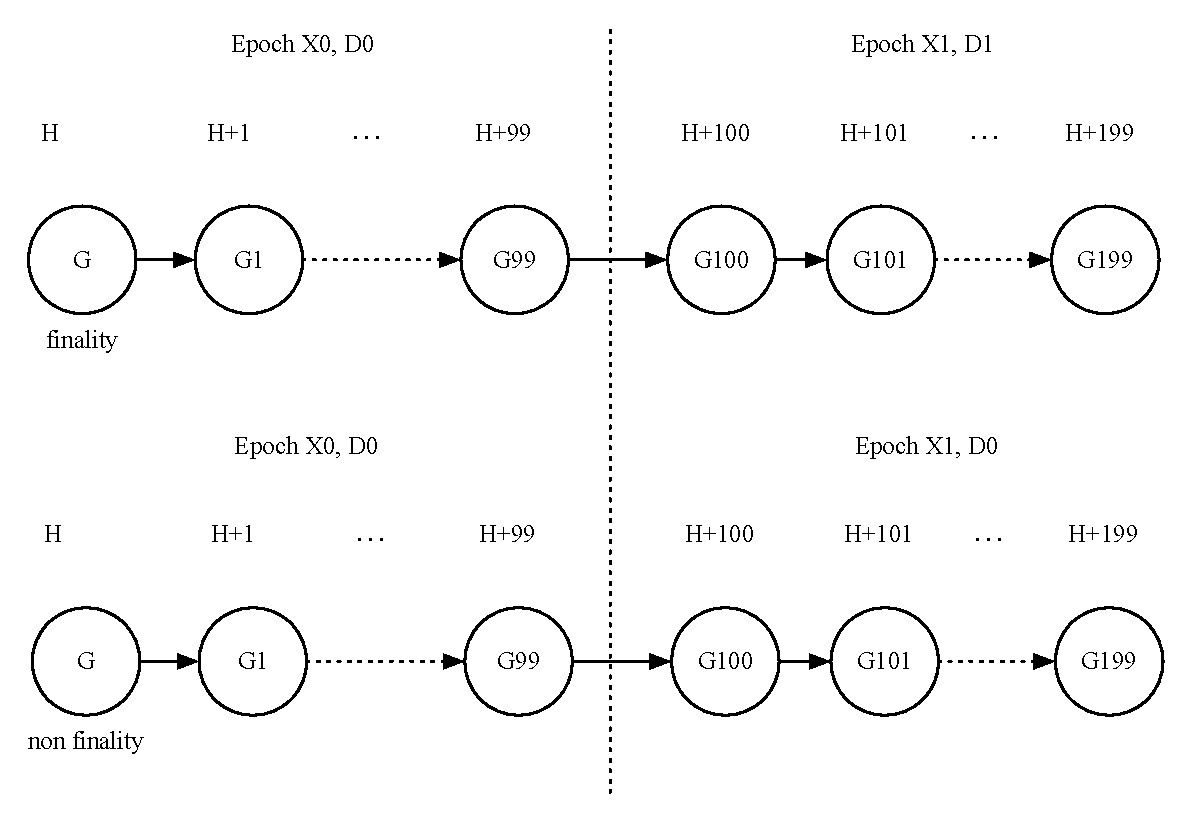
\includegraphics[width=10cm]{./figs/epoch}
\caption{Cambio de dinastías de validadores (asumiendo X = 100)}
\label{fig:epoch}
\end{figure}

A causa de las demoras en la red, el estado de finalidad del bloque G en cada uno de los nodos podría no ser el mismo cuando ocurre el cambio de dinastía. Por ello, haciendo referencia al conjunto de estrategias del validador dinámico Casper, será necesario el proceso de consenso de cada dinastía se complete en forma conjunta al conjunto de validadores de las dinastías previa y actual. Así, en cualquier dinastía, una cuenta elegible sólo podrá aplicar para el enlistamiento (o renuncia) en el conjunto de validadores de la dinastía D+2; así, cuando la dinastía D+2 esté vigente, podrá participar en el proceso de consenso del nuevo bloque.

\subsubsection{Proceso de consenso}
\label{pod:design:consensus}

Luego de que un nuevo bloque es propuesto, todos los participantes del conjunto de validadores de la dinastía actual podrán participar en una ronda de votos tolerante a faltas bizantinas, con el fin de determinar la legitimidad del bloque. Al comienzo de la votación, a cada validador que participe del consenso del bloque se le cobrará 2x (x es la proporción del bono incentivo) como depósito; a partir de ese momento se iniciará el proceso de votación en dos etapas que se describe a continuación:

\begin{itemize}

\item \textbf{En la primera etapa} será necesario que todos los validadores emitan el ticket de voto $Prepare$ por el nuevo bloque. Luego de emitir el ticket de voto $Prepare$, el validador recibirá un bono de $1.5x$. Si los validadores que poseen más de dos tercios del total de los depósitos tanto en la dinastía previa como la actual emiten los tickets de voto $Prepare$ por el nuevo bloque, ese bloque entrará en la segunda etapa de votación. Nótese que el propositor del nuevo bloque emite por defecto un ticket de voto $Prepare$ por el nuevo bloque.

\item \textbf{En la segunda etapa} se requiere que todos los validadores emitan tickets de voto $Commit$ para el nuevo bloque. Luego de la emisión de $Commit$, los validadores recibirán otro bono de $1.5x$. Si los validadores que poseen más de dos tercios del total de los depósitos tanto en la dinastía previa como la actual emiten los tickets de voto $Commit$ por el nuevo bloque, el mismo alcanzará el estado de finalidad.
\end{itemize}

Para acelerar el desarrollo del ecosistema, si la diferencia entre el timestamp de $Prepare$ y $Commit$ en el bloque $b$ y el timestamp del bloque $b$ excede $T$, esos tickets se considerarán expirados y se ignorarán.

\subsubsection{Elección de \textit{forks}}
\label{pod:design:fork}

El algoritmo PoD selecciona la cadena canónica de acuerdo al puntaje del bloque en cada \textit{altura}\footnote{\textit{Height} en inglés (N. del T.)}. Se seleccionará siempre el bloque que posea el mayor puntaje para unirse a la cadena canónica. El puntaje del bloque $b$ en la altura $h$ se calcula de este modo:

\begin{align}
Score(b, h) = \sum_{(b',h') \in children(b)}Score(b', h') + \sum committed~deposits~in~b
\end{align}
\noindent

Es decir, es la suma de los depósitos recibidos por este bloque y todos sus descendientes, correspondientes al ticket $Commit$, tal como se muestra en la \reffig{fig:fork_choice}.

\begin{figure}[h]
\centering
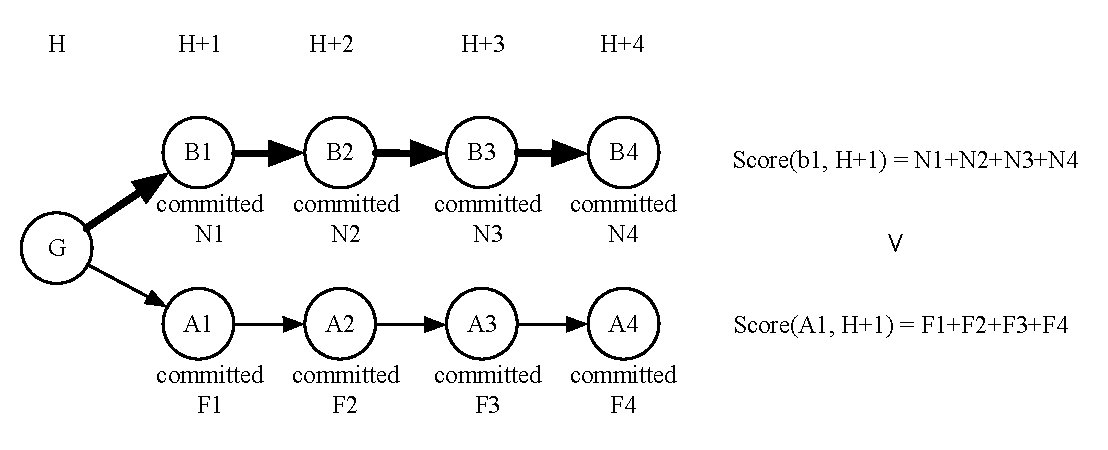
\includegraphics[width=12cm]{./figs/fork}
\caption{Fork Choice Example}
\label{fig:fork_choice}
\end{figure}

\subsubsection{Condiciones de confiscación}
\label{pod:design:vote}

Para evitar cualquier daño malicioso al proceso de consenso —que puede dar lugar a un fracaso en la finalización del proceso de consenso y a una obstrucción del desarrollo del ecosistema— PoD restringe las actividades de consenso de los validadores basándose en las condiciones mínimas de confiscación de Casper \cite{minimal_slash_rules}.

Asúmase que los tickets de voto $Prepare$ y $Commit$ en el proceso de consenso tienen la estructura siguiente:

\begin{itemize}
\item $Prepare(H, v, vs)$, donde $H$ es el valor hash del bloque actual; $v$ representa la altura del bloque actual; $vs$ representa la altura de un determinado bloque ancestral de $v$.

\item $Commit(H, v)$, donde $H$ es el valor hash del bloque actual; $v$ representa la altura del bloque actual.
\end{itemize}

El algoritmo PoD define las siguientes cuatro reglas básicas para el proceso completo de votación:

\begin{itemize}
\item Existe un orden estricto en el proceso de consenso de dos etapas de un bloque: sólo será posible para los validadores emitir los tickets de voto $Commit(H, v)$ de la segunda etapa cuando los depósitos totales de los tickets de voto $Prepare(H, v, vs)$ de la primera etapa alcanzan $2/3$.

\item Para bloques múltiples, no existen reglas que obliguen a esperar a que finalice un proceso de consenso antes de iniciar el siguiente. El consenso entrelazado está permitido siempre y cuando se lleve a cabo en cierto orden; sólo después de que la primera etapa de votación esté completa y la proporción de tickets de voto $Prepare(H, vs, vs’)$ alcance $2/3$ se podrán enviar los tickets $Prepare(H, v, vs)$ para los bloques descendientes, para asegurar la estabilidad de esta modalidad de consenso.

\item Para evitar que un nodo cualquiera pueda realizar votaciones interbloque maliciosas tomando ventaja del \textit{consenso entrelazado}, se requiere que luego de enviados los votos (H, w, u) basados en la altura de u, ningún voto Commit(H, v) se pueda enviar a aquellos bloques con una altura dentro del rango que va de $u$ a $w$, garantizando así la eficiencia y el orden en el proceso de consenso.

\item Con el fin de prevenir que los nodos puedan realizar el depósito de caución\footnote{\textit{Staking} en inglés (N. del T.)} en distintas ramas al mismo tiempo —lo que podría generar el problema de \textit{nada en juego}— se requiere que luego de emitir los votos $Prepare(H1, v, vs1)$ en una altura determinada, no sea posible emitir otro voto $Prepare(H2, v, vs2)$.
\end{itemize}

Una vez reportado y verificado, todo validador que viole las reglas citadas previamente recibirá una sanción y sus depósitos serán confiscados; de la confiscación, 4\% se repartirán entre quienes hayan reportado el incidente, y el resto será destruido.

\subsection{Análisis económico de la PoD}
\label{pod:economic}

\subsubsection{Análisis de incentivos}
\label{pod:economic:incentive}

Todo validador que participe del algoritmo PoD será recompensado con $1x$ NAS por cada bloque legítimo creado. En caso de no finalizar la etapa $Prepare$ e ingresar en la etapa $Commit$ debido a problemas de tráfico en la red o por comportamientos fraudulentos, el validador perderá $0.5x$ NAS. De ese modo, todo validador obtendrá una suma importante en concepto de ganancias de contaduría siempre y cuando mantenga una buena conexión de red y no se vea envuelto en actividades fraudulentas.

\subsubsection{Análisis de fraudes}
\label{pod:economic:fraud}

\subsubsection*{Ataque de doble gasto}
\label{pod:economic:fraud:double_spend}

Si se asume que un comerciante confirma una transacción y la envía cuando el nuevo bloque alcanza el estado de finalidad, entonces el costo mínimo a pagar por un fraude de compra sin costo por medio de un ataque de doble gasto bajo el consenso PoD se describe de este modo:

Primero, el estafador necesita incrementar su valuación Nebulas Rank para ingresar a los N principales\footnote{\textit{Top N} en inglés (N. del T.}, convertirse en validador mediante el pago de una suma $N$ de NAS como depósito de caución, y aplicar para la participación en la validación de bloques en la dinastía D+2.

Luego, el estafador necesita resultar seleccionado como propositor de un nuevo bloque a través del algoritmo pseudoaleatorio. En ese momento, el estafador propone dos nuevos bloques a la misma altura, de los cuales uno de los bloques tiene un valor hash $hash1$ y contiene una transferencia desde el estafador hacia el comerciante, mientras el otro bloque tiene un valor hash $hash2$ y contiene una transferencia desde el estafador hacia sí mismo.

Finalmente, para lograr que ambos bloques alcancen el estado de finalidad —como se muestra en la  \reffig{fig:double_spend}— el estafador necesita gastar $1/3$ del total de los depósitos en esa dinastía para sobornar a $1/3$ de los validadores y hacer que emitan tickets de voto $Commit$ para ambos bloques.

\begin{figure}[h]
\centering
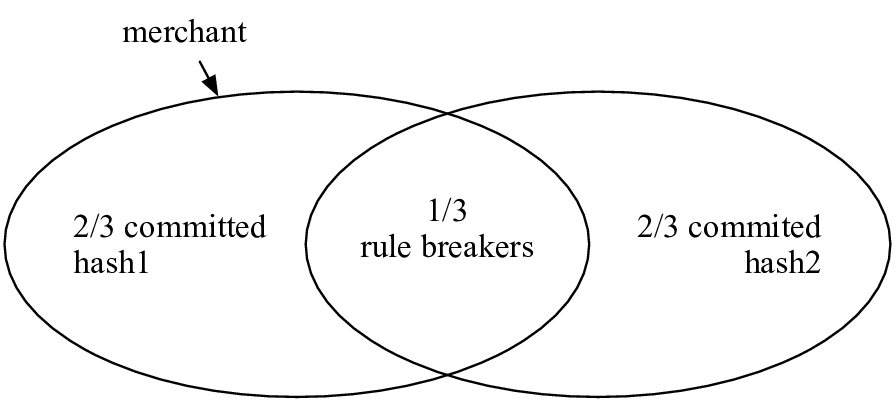
\includegraphics[width=7cm]{./figs/overlap}
\caption{Sanción financiera en casos de doble gasto}
\label{fig:double_spend}
\end{figure}

Por lo tanto, para completar un ataque exitoso de doble gasto, el estafador necesita gastar una determinada cantidad de energía y recursos financieros para incrementar su valuación Nebulas Rank (véase \refsec{subsec:robust}, “resistencia a la manipulación”) y entonces gastar al menos $1/3$ del valor total de los depósitos en esa dinastía para lograr que ambos bloques alcancen el estado de finalidad si es los suficientemente afortunado como para resultar selecto como propositor.

\subsubsection*{Ataque del 51\%}
\label{pod:economic:fraud:51attack}

En el consenso PoW, lanzar un ataque del 51\% implica poseer al menos el 51\% del poder de cómputo de la red entera. En el consenso PoS, es necesario contar con el 51\% del total de depósitos en caución. No obstante, en nuestro consenso PoD, un ataque del 51\% requiere poseer el 51\% de las cuentas del conjunto de validadores, lo que significa que un número significativo de cuentas de reputación necesitan ingresar a los \textit{N principales} de Nebulas Rank y realizar el pago de los depósitos de caución para cada una de las cuentas, por lo que un ataque de estas características es mucho más difícil en el algoritmo de consenso PoD.

\subsubsection*{Ataque de corto alcance}
\label{pod:economic:fraud:short_range_attack}

En PoD, los bloques de cada altura tienen plazo de caducidad para el consenso. Por lo tanto, es casi imposible completar un ataque de largo alcance en PoD, pero aún es posible lanzar ataques de corto alcance dentro del plazo de caducidad.

Si un atacante de corto plazo intenta fraguar la cadena $A$ para reemplazarla por la cadena $B$ con el fin de convertirla en el \textit{fork canónico} cuando los bloques a la altura de $H+1$ todavía se encuentran fuera del tiempo de expiración, necesitará asegurarse de que el puntaje del bloque $A1$ es mayor que el del bloque $B1$. El voto múltiple recibe sanciones muy fuertes, por lo que le resultará inevitable al atacante sobornar a los validadores; de otro modo, es imposible concretar un ataque de este tipo. Con el fin de demostrar la seguridad del algoritmo PoD, se muestran a continuación los costos que debe pagar el atacante para revertir un número dado de bloques.

Si el atacante planea revertir $B1$, el costo mínimo que debe pagar se describe en la  \reffig{fig:revert1}, que equivale al costo de un ataque de doble gasto. Si el atacante se convierte en un propositor de bloques a la altura de $H+1$, deberá sobornar a $1/3$ de los validadores en la dinastía $D0$ y convencerlos de realizar votaciones múltiples para lograr que $A1$ alcance el estado de finalidad, para lo cual el costo mínimo es de $1/3$ del total de los depósitos.

\begin{figure}[h]
\centering
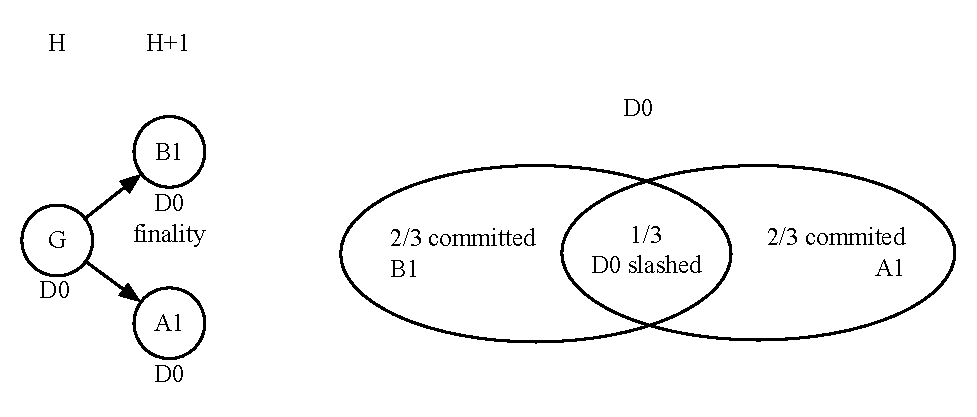
\includegraphics[width=11cm]{./figs/revert1}
\caption{Reversión de un bloque por parte de un atacante de corto plazo}
\label{fig:revert1}
\end{figure}

Asumiendo que $B1$ y $B2$ alcanzaron el estado de finalidad y las transacciones en los bloques han surtido efecto, si el atacante desea revertir $B1-B2$, se toman las dos circunstancias siguientes en consideración:

\begin{itemize}
\item La primera circunstancia se muestra en la \reffig{fig:revert2} (a): cuando las alturas $H+1$ y $H+2$ se encuentran en la misma época y dinastía, el atacante necesita sobornar a $1/3$ de los validadores en D0 para lograr que $A1$ alcance el estado de finalidad. Mientras tanto, ese $1/3$ de los validadores recibirán sanciones y sus depósitos serán totalmente confiscados. Durante la validación de $A2$, la suma de los depósitos equivale a $2/3$ de los depósitos en $A1$. En ese momento, si el atacante desea asegurar la misma cantidad de votos que en $B2$, debe sobornar al resto de los validadores sin cometer fraude, y perder al menos $3/3$ de los depósitos totales. Incluso en el caso de que el atacante tenga éxito en hacer esto, es imposible garantizar que el puntaje de $A1$ sea mayor que el de $B1$, con lo que el atacante enfrentará una alta probabilidad de fallar en el ataque.

\item La segunda circunstancia se muestra en la \reffig{fig:revert2} (b): cuando las alturas $H+1$ y $H+2$ están en distintas épocas y dinastías, el atacante necesita sobornar a $1/3$ de los validadores en $D0$ para lograr que $A1$ alcance estado de finalidad, y luego sobornar a $1/3$ de los validadores en $D1$ para lograr que $A2$ alcance también estado de finalidad, por lo que el atacante deberá perder al menos $2/3$ de los depósitos totales con el fin de completar tal ataque. En suma, para lanzar un ataque de corto plazo para causar la invalidación de dos bloques que han alcanzado el estado de finalidad, el atacante necesita pagar al menos $2/3$ de los depósitos totales.
\end{itemize}

\begin{figure}[h]
\centering
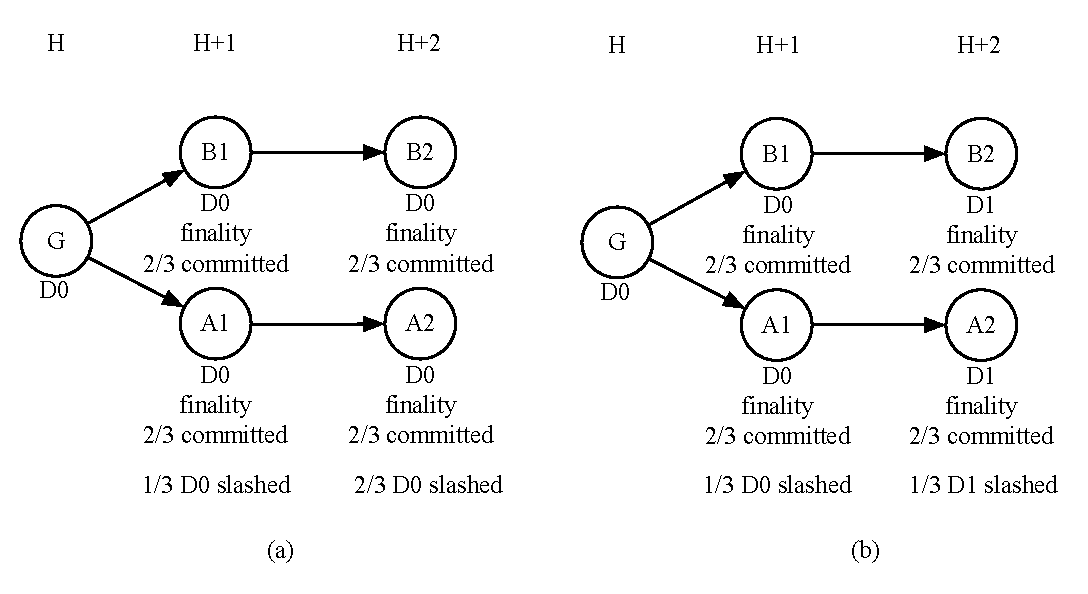
\includegraphics[width=11cm]{./figs/revert2}
\caption{Reversión de dos bloques mediante un ataque de corto plazo}
\label{fig:revert2}
\end{figure}

Si el atacante desea revertir $B1-B3$, como se muestra en la \reffig{fig:revert3}, necesitará primero sobornar a $1/3$ de los validadores en D0 para alcanzar la finalidad de $A1$ y luego sobornar a $1/3$ de los validadores de la dinastía $D1$ para alcanzar la finalidad de $A2$. Finalmente, el atacante necesita sobornar a los $2/3$ de los validadores en $D1$ para lograr la finalidad de $A3$. Resumiendo, perderá $4/3$ de los depósitos totales. Le resultará muy difícil preparar un ataque de estas características. Incluso si logra éxito en sus preparaciones, no puede garantizar que el puntaje de $A1$ sea mayor que el de $B1$. Por lo tanto, es muy probable que un ataque tal falle.

\begin{figure}[h]
\centering
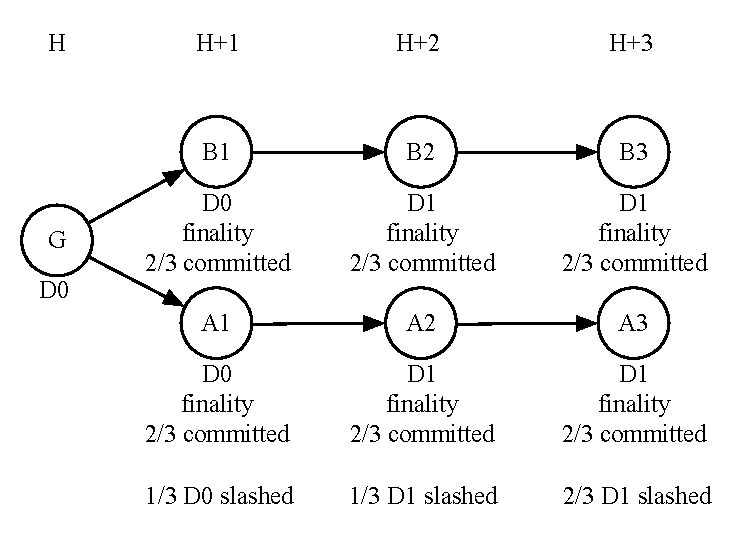
\includegraphics[width=7.5cm]{./figs/revert3}
\caption{Reversión de tres bloques mediante un ataque de corto plazo}
\label{fig:revert3}
\end{figure}

En general: si un atacante desea revertir $B1-BN$ —en donde $N$ está limitado por el plazo de vencimiento del consenso del bloque y por ende no puede ser un número muy grande— cuando $N = 3$, el total de los depósitos de todos los validadores de la dinastía actual serán completamente confiscados. Así, cuando $N >= 4$, será imposible completar el ataque para lograr que el puntaje de $B1$ sea mayor que $A1$ y así revertir $B1-BN$. No tendría sentido alguno un ataque de estas características.